\documentclass[12pt,a4paper]{article}
\usepackage[utf8]{inputenc}
\usepackage{amsmath}
\usepackage{amsfonts}
\usepackage{amssymb}
\usepackage{graphicx}
\usepackage{lmodern}
\usepackage{caption}
\usepackage[left=2cm,right=2cm,top=2cm,bottom=2cm]{geometry}
\author{Michael Morgan (GLJ Petroleum Consultants)}
\title{Stochastic modelling of oil and gas economics}
\begin{document}
\maketitle

\section{Background preparation}
Differential equations, stochastic modelling, statistical models, time series analysis, econometrics, numerical methods. Some knowledge of financial mathematics and asset pricing would be great. 



\section{Overview: stochastic economic models}

\begin{figure}[h]
\centering
	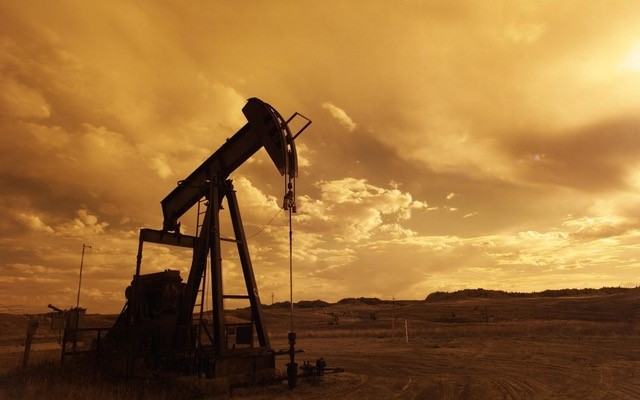
\includegraphics[width=0.6\linewidth]{oil-pump.jpg}
\caption*{Modelling uncertainty in oil and gas economies.}
\label{fig:oil-pump}
\end{figure}

Many aspects of the oil and gas industry are subject to economic uncertainty: success in finding oil and gas reserves is highly unpredictable, productivity of an individual well can change in seemingly random ways, markets for products can move unexpectedly, future prices and interest rates are unknown, among other challenges. Useful economic models need to account for these uncertainties. Stochastic models provide an approach to these problems by treating certain unknown parameters as random variables and performing an in-depth analysis that takes into account this uncertainty.

Stochastic differential equations (SDEs) are one useful method whose application are of interest to oil and gas economic problems. As most economic analysis is currently conducted using deterministic discounted cash flow models, there is much scope of innovation and experimentation. In particular, there is much scope for improving how uncertainty is mathematically modelled. In these project, we are interested four different general areas:
\begin{itemize}
\item Econometrics
\item Real Options Analysis
\item Geographic Correlation and Temporal Uncertainty
\item SDE Solutions to PDEs
\end{itemize}




\section{Problem Descriptions}

The four general areas can be approached by specific problems, for which we are looking for specific outcomes.  Participants are welcome to try all these problems but are encouraged to choose a subset of these problems and develop more comprehensive solutions complete with specific numeric solutions and supporting code.  The use of open source software is preferred, with Python, R, Stan and Octave being particularly well suited to these problems.


\subsection{Econometrics}

{\bf Model construction and estimation of parameters for Canadian energy commodity prices }

Most econometric analysis has used price series external to Canada. It is common to consider the price of West Texas Intermediate (WTI) oil or of gas traded at Henry Hub. However, Canadian producers most often receive revenues based on the price of oil at various refineries in Edmonton or on the price of gas at either the AECO trading hub or at Station 2 in British Columbia. A further complication is the relatively large amount of heavy oil produced within Alberta which is sold at a discount to prices of light oil. These local hydrocarbon prices are related to each other and to world benchmarks (such as WTI) but do not necessarily share the same variance or other model structures.

Current practice often models Canadian prices to be simple linear functions of world benchmark prices. However, such models do not allow different mean reversion rates, volatilities or correlations, all of which may be necessary to reflect fundamental physical and economic differences specific to the Canadian market. Exploring price models suitable for Canadian producers would provide improvements in the ability to properly assess price inter-dependencies and uncertainties.

Data for various Canadian price series can be provided by GLJ Publications.

A successful solution would propose an analytical framework suited to the observed dynamics of Canadian energy commodity prices; statistical work supporting the inclusion or exclusion of various factors or terms; calculation of best estimate parameters; forecasts showing equi-probable future outcomes and any computer code required for these calculations.


\subsection{Real Options Analysis}

{\bf Economics of constructing gas processing plants that extract more liquid hydrocarbons }

In designing gas processing plants an important factor is the degree to which various higher weight hydrocarbons are separated from methane. This is commonly done by chilling the gas until the higher weight hydrocarbons condense and can be removed as a liquid. As different hydrocarbons have different boiling points, the relative amount of condensation of each hydrocarbon can be controlled by careful choice of temperature. Operators often consider increasing the recovery of higher weight hydrocarbons by constructing gas plants that operate at lower temperatures. This allows the hydrocarbons to be sold as liquids (taking advantage of higher liquids prices) instead of a gas. However, running gas plants at lower temperatures increases operating costs. Moreover, the operating temperature is primarily determined by the design and construction of the plant while the relative value of hydrocarbon liquids to gases is determined by spot and futures markets and is under constant change.

The choice of plant operating temperature can be viewed as a real option. The value of this real option will be determined by whether various hydrocarbon species (ethane, propane, butane, pentane, etc.) are sold as separate liquids or sold within the gas stream, by the incremental cost of constructing plants capable of operating at lower temperatures and by the incremental costs of operating at those lower temperatures. As the prices of various hydrocarbon species are interdependent (and likely co-integrated), a suitable commodity price model will likely be needed.

Constructing a model of the real option of gas plant operating temperature would improve the ability of investors to weigh the relative merits of various plant designs, thereby maximizing the economic return of investments.

Historical data for various hydrocarbon prices series can be provided by GLJ Publications, simplified models for hydrocarbon yields and plant costs can be provided by GLJ Petroleum Consultants.

A successful solution would propose an analytical model that captures the major physical relationships between liquid yield, operating temperatures and operating cost; inclusion of a simplified co-integrated price model; calculation of the optional value of plant construction as a function of input parameters, including temperature and any computer code required for these calculations.


\subsection{Geographic Correlation and Temporal Uncertainty}

{\bf Pipeline supply with discrete correlated declining input sources }

Nearly all energy resources are spatially correlated and aggregated using fixed infrastructure. Whether this is the sunlight available for a solar panel, the wind to power a turbine or productivity of a gas well, high output point sources are likely to be located near other high output sources. Within the mining industry such correlations are often characterized using various geostatistical descriptions like variogram models. Such models often use static outputs: the relative presence of minerals for example. However, energy supplies often also have a temporal quality. The wind speed changes throughout the day and gas wells typically produce at higher rates early in their lives. Thus, wise investment decisions on fixed infrastructure will need to consider both spatial and temporal patterns.

It would be beneficial to have a model for pipeline supply that considers a catchment area within which discrete input sources are located (ie gas wells). These input sources are not constant: they decline over time according to uncertain spatially correlated parameters. Such a model should calculate the distribution of number of point sources required, and the pace of adding them, to maintain a constant supply to the pipeline. Such a model should also consider how the distribution changes with increasing certainty, both in terms of the underlying (spatially varying) productivity of the area and in terms of the uncertainty of the decline parameters.

Such a model for pipeline supply would be beneficial when considering development within relatively untested areas, thereby better informing investment decisions and development strategies.

Historical data for various catchment areas can be provided by GLJ Petroleum Consultants.

A successful solution would propose an analytical framework; statistical work supporting the choice of spatial and temporal models; forecasts of various development scenarios, the distribution of point sources required to maintain a constant supply and the impact of certainty of model parameters on this distribution; and any computer code required for these calculations.



\subsection{SDE Solutions to PDEs}

{\bf Stochastic solutions to partial differential equations commonly used to model production from oil and gas wells }

There are two main techniques to model production from oil and gas wells: physics-based 3D simulations and approximations based on simple partial differential equations (PDEs). Simple PDE approximations are the more commonly used for economic calculations, especially those with compact analytical solutions. For example, late life wells produced with a constant pressure are often modelled using a simple exponential relationship, $\frac{dq}{dt} = -D q$ where $q$ is the flow rate and $D$ is a constant rate of decline. The parameters of these models cannot be precisely determined a priori, nor can they be estimated with precision due to the difficulty in precisely controlling producing conditions for accurate flow measurements. As such, forecasts are uncertain. 

Our goal here is to model the parameters as stochastic processes and solve the resulting stochastic differential equations using Ito's Lemma. These can then be used to compare with data from actual wells to evaluate how well these stochastic models are working.

Common PDEs used to forecast production include the following:

Arps:

$$\frac{dq}{dt} = - \left( \frac{D_i}{q_1^b} \right) q^{b+1}$$

Power Law Exponential:

$$ \frac{dq}{dt} = - \left( D_\infty + D_1 t^{-(1-n)} \right) q$$

Stretched Exponential:

$$\frac{dq}{dt} = -\left( \frac{n}{t} \left( \frac{t}{\tau}\right)^n \right) q$$

Logistic Growth:

$$\frac{dq}{dt} = -\left( \frac{a-an+(1+n)t^n}{t\left(a+t^n\right)} \right) q$$

Duong:

$$\frac{dq}{dt} = -\left( mt^{-1}-at^{-m}\right) q$$

Stage two of this sub-problem is to define stochastic process to model net cash flow, including royalties. Net cash flow will be revenue minus expenses and taxes. Revenues will be a simple multiple of instantaneous volume produced and instantaneous price. Operating expenses will be a linear function of time plus a simple multiple of instantaneous volume produced and processing cost. Royalties (ie taxes) will be function of average rate and price over an accounting interval, typically a month.

Historical production data and typical economic parameters, including royalty models, can be provided by GLJ Petroleum Consultants.

A successful solution would propose analytical stochastic solutions to a selection of the common PDEs models; calculation of best estimate parameters; forecasts showing equi-probable future production outcomes; forecasts showing the distribution of expected future revenues and any computer code required for these calculations.



\end{document}



